\documentclass[12pt]{article}

\usepackage[sorting=none]{biblatex}
\usepackage{mystyle}
\setlength{\parskip}{1em}

\addbibresource{biblio.bib}


\begin{document}
	%%% Maketitle metadata
\newcommand{\horrule}[1]{\rule{\linewidth}{#1}} 	% Horizontal rule

\title{
	\vspace{-1in}
	\usefont{OT1}{bch}{b}{n}
	\normalfont \normalsize \textsc{CVPR - Exam} \\ [25pt]
	\horrule{0.5pt} \\[0.4cm]
	\huge Project 2 report \\
	\horrule{2pt} \\[0.5cm]
}
\author{
	\normalfont 								\normalsize
	Patrick Indri\\[-3pt]		\normalsize
	\selectlanguage{english}
	\today
}
\date{}


	\maketitle

  \section*{Problem statement}

  The assignment requires the implementation of an image classifier based on the bag-of-words approach. The provided dataset, taken from \cite{lazebnik2006beyond}, consists of \( \approx 4500 \) images from \( 15 \) categories. The dataset is already divided into a test and a training set. The task has been carried out using the Python programming language. Please refer to the provided \texttt{Readme.md} for quick details on how the project is organised into folders.


  \subsection*{Disclaimer on \texttt{OpenCV}}

  Since version 3.0, OpenCV no longer includes widely used patented algorithms such as SIFT and SURF. However, those algorithms are included as "extra modules" in the \href{https://github.com/opencv/opencv_contrib}{opencv\_contrib} GitHub repository. The library must be compiled from source, specifying the inclusion of the "non free" algorithms. As an alternative, one could use the \href{https://opencv-python-tutroals.readthedocs.io/en/latest/py_tutorials/py_feature2d/py_orb/py_orb.html}{ORB algorithm}, a free alternative to SIFT or SURF.



  \section*{1. Visual vocabulary}
  
  The first step requires the construction of a visual vocabulary. Images are read using a generator that yields the image path and its folder name (that is, its class label). Then, for each of the images in the training set, the SIFT algorithm is used to extract keypoints and compute descriptors. The number of features to be retained can be passed as an argument, but was left at the default value (which, incidentally, is not clearly specified by the documentation). The descriptors and the labels are associated to an image ID and everything is stored in a Pandas \texttt{Dataframe}. As required, \( 1000000 \) descriptors are sampled and clustered using \( k \)-means. The \texttt{sklearn.cluster.KMeans} function returns an object containing info on the clusters including the coordinates of the centroids. Different numbers of clusters have been tested.
  

  \subsection*{Results}

	\begin{table}[H] 
		\centering
		\caption*{Training set, descriptors dataframe.}
		\rowcolors{1}{}{gray!10}
		\begin{tabular}{lll}
			\toprule
      image\_id & descriptor & label \\
      \midrule
      3 &  [8.0, 2.0, 46.0, 42.0, 2.0, 19.0, ...    &  Industrial \\
      3 &  [18.0, 2.0, 0.0, 0.0, 4.0, 49.0, ...     &  Industrial \\
      3 &  [10.0, 1.0, 0.0, 20.0, 4.0, 14.0, ...    &  Industrial \\
      3 &  [57.0, 33.0, 121.0, 3.0, 0.0, 1.0, ...   &  Industrial \\
      4 &  [16.0, 20.0, 8.0, 4.0, 24.0, 17.0, ...   &  Industrial \\
      4 &  [35.0, 9.0, 11.0, 27.0, 0.0, 0.0, ...    &  Industrial \\
      4 &  [38.0, 0.0, 1.0, 9.0, 4.0, 0.0, 0.0, ... &  Industrial \\
			\bottomrule
		\end{tabular}
	\end{table}



  \section*{2. Histogram representation}

  Each of the \( k \) cluster centroids is interpreted as a visual word, thus constituing a vocabulary. Training set images can now be represented as histograms having \( k \) bins: for each image, the code cycles through the list of its descriptors and increases by one the bin correspoinding to the closest word in the vocabulary (that is, the closest centroid). Euclidian norm is used to compute all the distances while \texttt{np.argmin} is used to identify the smallest one. Since different images might have a different number of descriptors, the histograms are then normalised to make them comparable with each other. The normalised histograms are added as a column to the descriptors dataframe.

  \subsection*{Results TBD}

	\begin{table}[H] 
		\centering
		\caption*{Training set, descriptors dataframe.}
		\rowcolors{1}{}{gray!10}
		\begin{tabular}{lll}
			\toprule
      image\_id & descriptor & label \\
      \midrule
      3 &  [8.0, 2.0, 46.0, 42.0, 2.0, 19.0, ...    &  Industrial \\
      3 &  [18.0, 2.0, 0.0, 0.0, 4.0, 49.0, ...     &  Industrial \\
      3 &  [10.0, 1.0, 0.0, 20.0, 4.0, 14.0, ...    &  Industrial \\
      3 &  [57.0, 33.0, 121.0, 3.0, 0.0, 1.0, ...   &  Industrial \\
      4 &  [16.0, 20.0, 8.0, 4.0, 24.0, 17.0, ...   &  Industrial \\
      4 &  [35.0, 9.0, 11.0, 27.0, 0.0, 0.0, ...    &  Industrial \\
      4 &  [38.0, 0.0, 1.0, 9.0, 4.0, 0.0, 0.0, ... &  Industrial \\
			\bottomrule
		\end{tabular}
	\end{table}



  \section*{3. Nearest Neighbour classifier}

  Test images can be classified using a nearest neighbour classifier. In particular, histograms for the test images are computed as previously done for the training set (not that, in this step, the visual vocabulary must not be rebuilt: the training one is used to compute the histograms). Then the histogram of a test image is compared with all the training histograms: the classifier assigns to the test image the label corresponding to the closest train histogram. Distances between histograms can be computed using the \textit{Earth Mover Distance}, implemented in \texttt{scipy.stats.wasserstein\_distance}.
  
  It should be noted that the histograms for the test set are precomputed once and then fed to different classifiers, reducing classification overhead. An alternative approach would be to designate the computation to each of the classifiers. All the implemented classifiers present a similar interface, accepting the train and test dataframes as inputs and returning both the true and the predicted labels for the test set.

  \subsection*{Results}

  \begin{figure}[H]
    \centering
    \caption*{Confusion matrix (for \( k = 48 \)) and accuracy for different values of \( k \).}
    \raisebox{-6em}{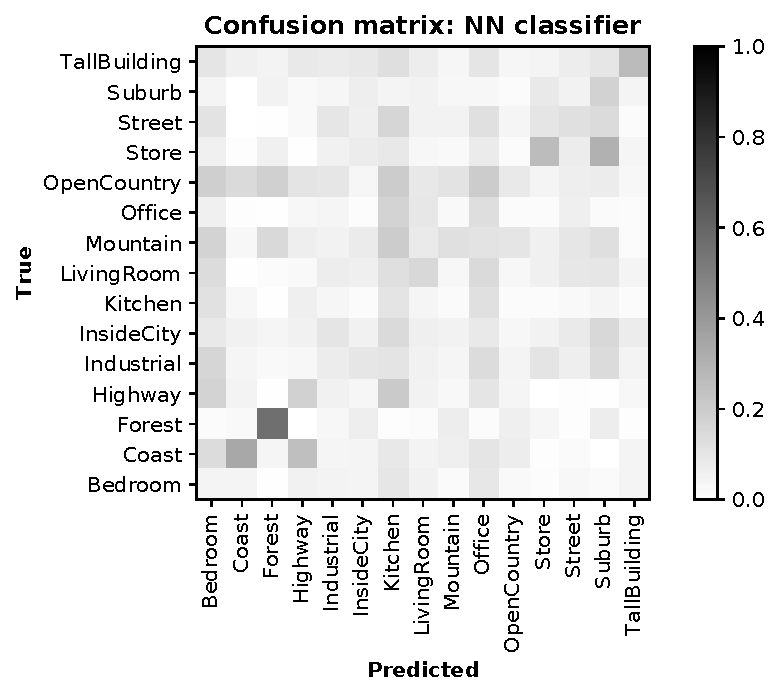
\includegraphics[width=.55\linewidth]{img/nn.pdf}}
    \quad\quad\quad
		\rowcolors{1}{}{gray!10}
    \begin{tabular}[b]{cc}
			\toprule
      Clusters (\( k \)) & Accuracy \\
      \midrule
      24  & tbd \\
      48  & 0.16 \\
      96  & tbd \\
      192 & tbd \\
      \bottomrule
    \end{tabular}
  \end{figure}

  The plot and the table above synthesize the results of the nearest neighbour classification. The accuracy values and the confusion matrix show that this classifier does not perform well on the test set. It performs significantly better than the random classifier (\( \approx 7\% \) accuracy) and the naive classifier that always predicts the most frequent class (\( \approx 10\% \) accuracy); however, all classes but the \textit{forest} one seem to be randomly predicted.



  \section*{4. and 5. Linear SVM}

  In this steps a multi-class Support Vector Machine classifier with linear kernel was implemented. In particular, the SVM is implemented using the one-vs-rest approach, training a binary SVM for each of the classes to separate it from the remaining ones. The normalised histograms constitute the input vectors. To overcome the unclassifiable regions problem, distance from the separating hyperplanes is used as the classification criterion: the image is assigned to the class corresponding to the most distant SVM separating hyperplane.

  Concerning implementation details, the SVM linar classifier is provided by \texttt{sklearn.svm.SVC} using \texttt{kernel = linear}. The distance from the hyperplane is computed, as suggested by the documentation, taking the value of the classifier \texttt{decision\_function} on the histogram and dividing it by the classifier \texttt{coef\_}.

  \subsection*{Results}

  \begin{figure}[H]
    \centering
    \caption*{Confusion matrix (for \( k = 48 \)) and accuracy for different values of \( k \).}
    \raisebox{-6em}{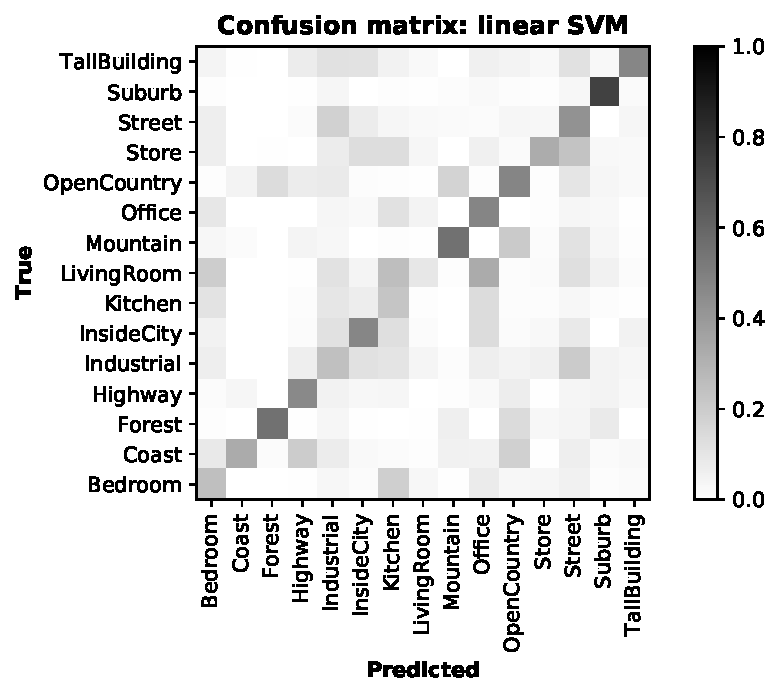
\includegraphics[width=.55\linewidth]{img/linsvm.pdf}}
    \quad\quad\quad
		\rowcolors{1}{}{gray!10}
    \begin{tabular}[b]{cc}
			\toprule
      Clusters (\( k \)) & Accuracy \\
      \midrule
      24  & tbd \\
      48  & 0.39 \\
      96  & tbd \\
      192 & tbd \\
      \bottomrule
    \end{tabular}
  \end{figure}



  \section*{6. and 7. Gaussian kernel SVM}

  A multi-class SVM classifier with Gaussian kernel was implemented as well. In this case, the \texttt{sklearn.multiclass.OneVsRestClassifier} function, fed with \texttt{skearn.svm.SVC(kernel = precomputed)}, is employed to build the classifier. In order to fit such classifier on the training data, the Gram matrix of the training set must be provided as an argument. The proposed implementation of the Gram matrix takes two sets of histograms as arguments; by default it uses a Gaussian kernel and the \( \chi^2 \) distance, but Earth Mover Distance was tested as well. The predictions are carried out passing the Gram matrix build over both train and test histograms to the classifier.


  \subsection*{Results}

  \begin{figure}[H]
    \centering
    \caption*{Confusion matrix (for \( k = 48 \)) and accuracy for different values of \( k \).}
    \raisebox{-6em}{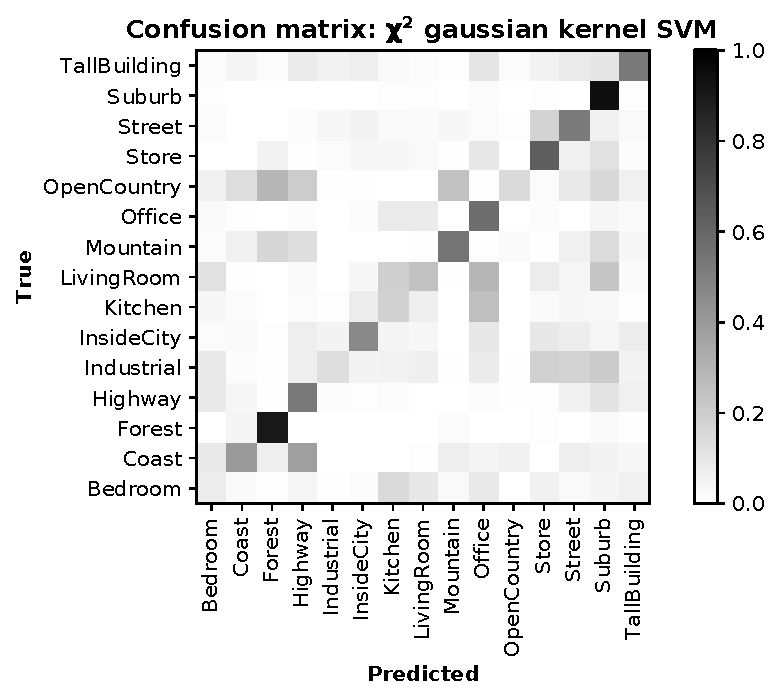
\includegraphics[width=.55\linewidth]{img/gaussvm.pdf}}
    \quad\quad\quad
		\rowcolors{1}{}{gray!10}
    \begin{tabular}[b]{cc}
			\toprule
      Clusters (\( k \)) & Accuracy \\
      \midrule
      24  & tbd \\
      48  & 0.42 \\
      96  & tbd \\
      192 & tbd \\
      \bottomrule
    \end{tabular}
  \end{figure}

  \textcolor{red}{0.21 for edm distance with k = 48}


  
  \section*{8. Error Correcting Output Code SVM}

  Error Correcting Output Code is an ensemble method for multi-class classification. The approach, detailed in \cite{dietterich1994solving} and \cite{james1998error}, combines many binary classifiers in order to solve a multi-class problem. In particular, each class is represented by a binary string where the length of the string corresponds to the number of binary classifiers; such representation is stored in a binary coding matrix:

	\begin{table}[H] 
		\centering
		\caption*{Example: coding matrix using 15 classifiers for 10 classes.}
		\rowcolors{1}{}{gray!10}
		\begin{tabular}{crrrrrrrr}
			\toprule
      Class & \( Z_1 \) & \( Z_2 \) & \( Z_3 \) & \( Z_4 \) & \( Z_5 \) & \( Z_6 \) & \( \dots \) & \( Z_{15} \) \\
      \midrule
      0 & 1 & 0 & 1 & 0 & 0 & 1 & \dots & 1 \\
      1 & 0 & 0 & 1 & 0 & 1 & 1 & \dots & 1 \\
      \( \vdots \) & & & & &  & & & \\
      9 & 1 & 0 & 0 & 1 & 1 & 0 &\dots & 0 \\
			\bottomrule
		\end{tabular}
	\end{table}

  Following the proposed example, the first binary classifier \( Z_1 \) should learn the representation \( 1 \) for class \( 0 \), representation \( 0 \) for class \( 1 \), and so on. Once all the classifiers have been fitted they can be evaluated on a test observation to produce a bit representation of it. The class whose expression (in the coding matrix) is the closest to the test observation representation is chosen as the predicted label.

  The coding matrix can be manually constructed to maximise expressiveness (guaranteeing a good separation between the classes representations) but, particularly for a large number of classes, a randomly generated matrix performs well. As the authors of \cite{james1998error} argue, the main benefit of the approach is variance reduction via model averaging, which is comparable for optimally constructed and random coding matrices. The approach is not prone to overfitting and a large number of classifiers provides better results.

  In the proposed implementation the coding matrix is randomly generated and the distance between binary strings is computed using the Hamming distance.


  \subsection*{Results}

  Plot varying B.

  \begin{figure}[H]
    \centering
    \caption*{Confusion matrix (for \( k = 48 \)) and accuracy for different values of \( k \). \( 100 \) binary classifiers.}
    \raisebox{-6em}{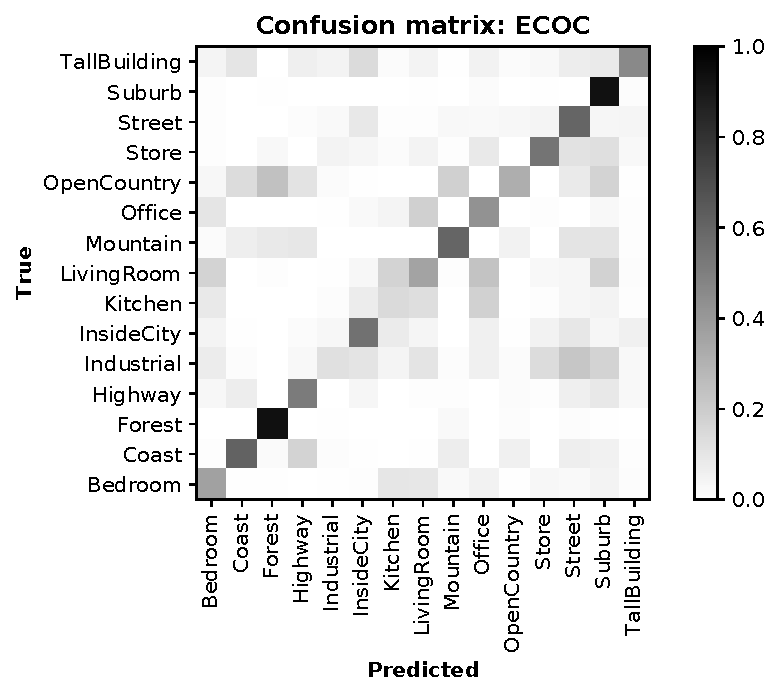
\includegraphics[width=.55\linewidth]{img/ecoc.pdf}}
    \quad\quad\quad
		\rowcolors{1}{}{gray!10}
    \begin{tabular}[b]{cc}
			\toprule
      Clusters (\( k \)) & Accuracy \\
      \midrule
      24  & tbd \\
      48  & 0.48 \\
      96  & tbd \\
      192 & tbd \\
      \bottomrule
    \end{tabular}
  \end{figure}




\renewcommand*{\refname}{References}
\printbibliography


\end{document}
